\subsection{AHTR Moltres Temperature Model}
\begin{frame}
    \frametitle{AHTR Temperature Model}
    \begin{block}{Moltres \cite{lindsay_introduction_2018}}
        \begin{itemize}
			\item An application built on the \gls{MOOSE} framework, for the simulation of 
            MSRs
            \item \gls{MOOSE} \cite{gaston_moose:_2009} is an open source finite
			element framework written in \texttt{C++} that
			relies on Libmesh and PETSc for meshing and PDE solving capabilities
			\item Moltres can run transient, implicitly coupled
			neutronics/thermal-hydraulics simulations
			\begin{itemize}
				\item Multi-group neutron diffusion (arbitrary no. of groups)
				\item Delayed neutron precursor decay (with advection)
				\item Incompressible Navier-Stokes for temperature
				advection-diffusion
			\end{itemize}
		\end{itemize}
    \vspace{-0.2cm}
    \end{block}
    \begin{block}{AHTR Temperature Model with Moltres}
        \begin{itemize}
            \item Captures thermal feedback effects, absent from the purely neutronics OpenMC
            simulations
            \item I model the steady-state temperature of a 2D x-y AHTR cross-section
            \item Assumptions: conductive heat transfer, heat removal by uniform 
            salt flow in coolant regions
        \end{itemize}
    \end{block}
\end{frame}

\begin{frame}
    \frametitle{AHTR Temperature Model Setup}
    \begin{block}{Steps to produce Moltres AHTR Temperature Model}
        \begin{itemize}
          \item OpenMC neutronics model produces group constants data (various macroscopic 
          neutron cross sections, neutron diffusion coefficient, etc. )
          \item Mesh generation
          \item Run Moltres model to calculate temperature distribution 
          (accepts group constants data and mesh)
        \end{itemize}
    \end{block}
    Using these group constants and mesh, Moltres then solves for the flux and temperature 
    based on the neutron diffusion equation coupled with temperature advection due to coolant flow.
    
    For successful AHTR Moltres simulation, I must establish \textbf{suitable spatial and
    energy homogenization that preserves accuracy} while maintaining an acceptable
    runtime
\end{frame}

\begin{frame}
    \frametitle{AHTR Temperature Model Energy Homogenization}
        \begin{block}{Energy Homogenization}
            \begin{table}[]
                \centering
                \begin{minipage}[c]{0.6\textwidth}
                    \centering
                    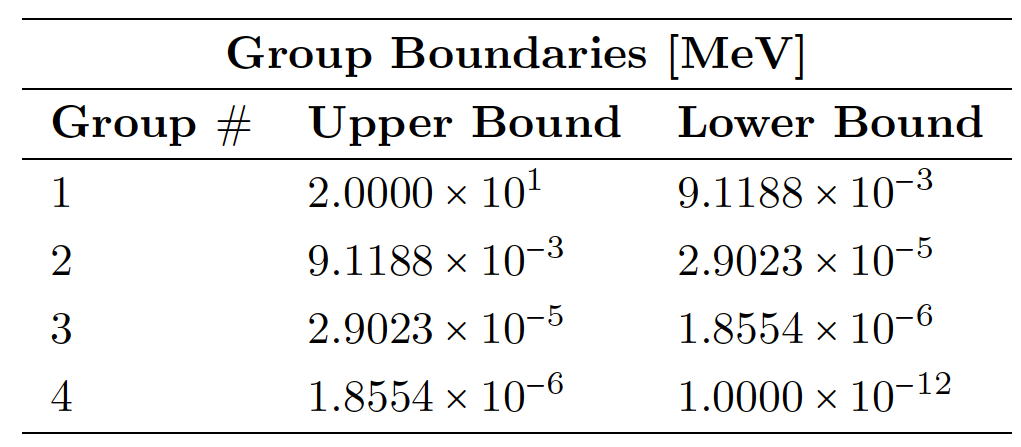
\includegraphics[width=0.8\linewidth]{figures/ahtr-energy-discr.png}
                \end{minipage}\hfill
                \begin{minipage}[c]{0.4\textwidth}
                \caption{4-group energy structures for AHTR geometry 
                derived by \cite{gentry_development_2016}.}
            \end{minipage}
            \end{table}
        \end{block}
\end{frame}

\begin{frame}
    \frametitle{AHTR Temperature Model Spatial Homogenization}
        \textbf{Fuel assembly 61 cell discretization}: inter-assembly FLiBe, 
        Y-shaped graphite structure, control rod slot FLiBe, graphite spacers, 
        each diamond shape section's inter-plank FLiBe (3), each graphite plank (18), 
        and each fuel stripe (36)
    \begin{figure}[]
            \centering
            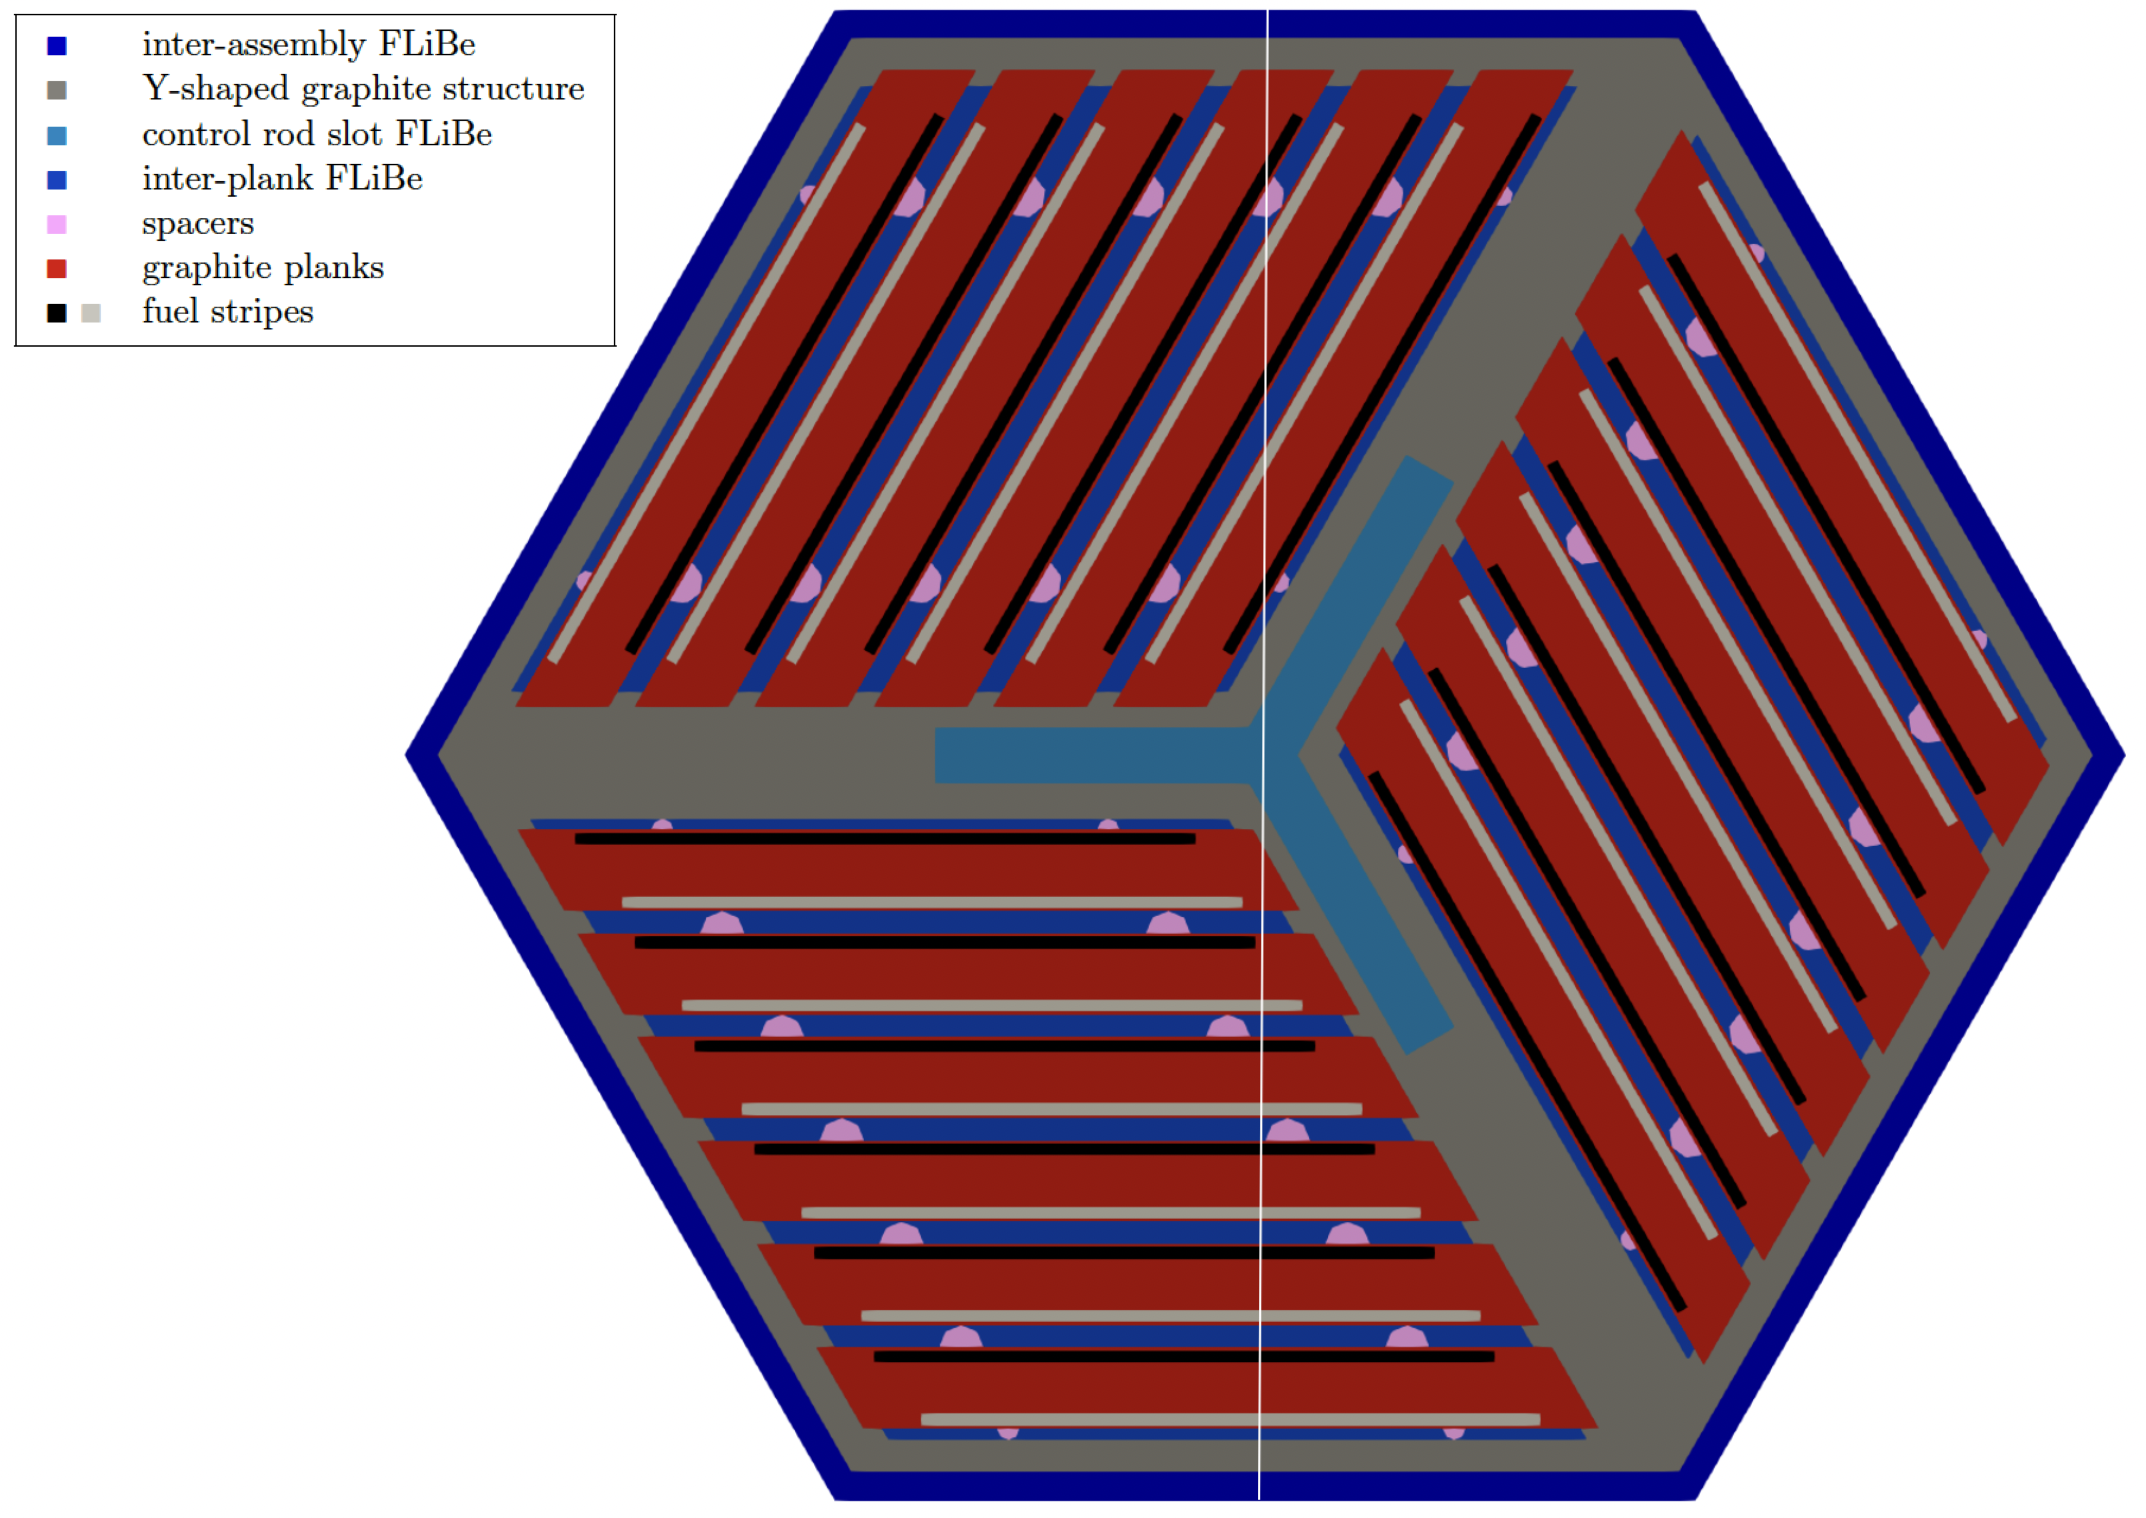
\includegraphics[width=0.65\linewidth]{figures/assembly_mg_pres.png}
        \caption{AHTR assembly spatial homogenization for group constant generation.}
    \end{figure}
\end{frame}

\subsection{Key Neutronics Parameters Verification}
\begin{frame}
    \frametitle{AHTR Temp Model Key Neutronics Parameter Verification}
    I \textbf{verify acceptable spatial homogenization and energy discretization} by 
    comparing key neutronics parameters (KNPs) between: 
    \begin{itemize} 
        \item OpenMC simulation with continuous energy and TRISO-level spatial fidelity
        \item Moltres simulation with 4-group energy and spatial homogenization
    \end{itemize}
    \textbf{KNPs}: $k_{eff}$, reactivity coefficients, flux distribution, and neutron 
    spectrum
    \begin{itemize}
        \item All comparisons are to verify that the Moltres model is replicating the 
        OpenMC model's neutronics correctly
    \end{itemize}
    \textbf{Reactivity coefficients and flux distribution}
    \begin{itemize}
        \item Ensure that \textbf{Moltres accurately calculates the AHTR's temperature 
        distribution}
        \item Reactivity coefficients capture temperature reactivity feedback on the flux
        \item Moltres source term is dependent on flux 
    \end{itemize}
\end{frame}

\begin{frame}
    \frametitle{Key Neutronics Parameter Verification Summary}
    OpenMC vs Moltres models \textbf{key observations} 
    \begin{itemize}
        \item 216 pcm reactivity diff 
        \item Good agreement in reactivity coefficients and 4-group neutron spectrum
        \item Good agreement in overall flux but larger flux diffs at specific points
    \end{itemize}
    Explanations: 
    \begin{itemize}
        \item Reactivity and flux differences due to Moltres' \textbf{neutron diffusion 
        method} 
        \item Differences in reactivity and flux at specific points might result in 
        \textbf{slightly inaccurate temperatures at certain points}
        \item Since the reactivity coefficients and overall flux distribution 
        are in agreement, OpenMC's group constants are \textbf{sufficiently accurate} 
        to calculate and gain an \textbf{overall perspective} of the AHTR's temperature 
        distribution
    \end{itemize}
    Methodology 
    \begin{itemize}
        \item I use this same Moltres model verification method for the AHTR geometries 
        used for optimization 
    \end{itemize}
\end{frame}

\subsection{AHTR Temperature Model Results}
\begin{frame}
    \frametitle{AHTR Temperature Model Results}
    \begin{columns}
        \begin{column}{0.6\textwidth}
            \begin{figure}[]
                \centering
                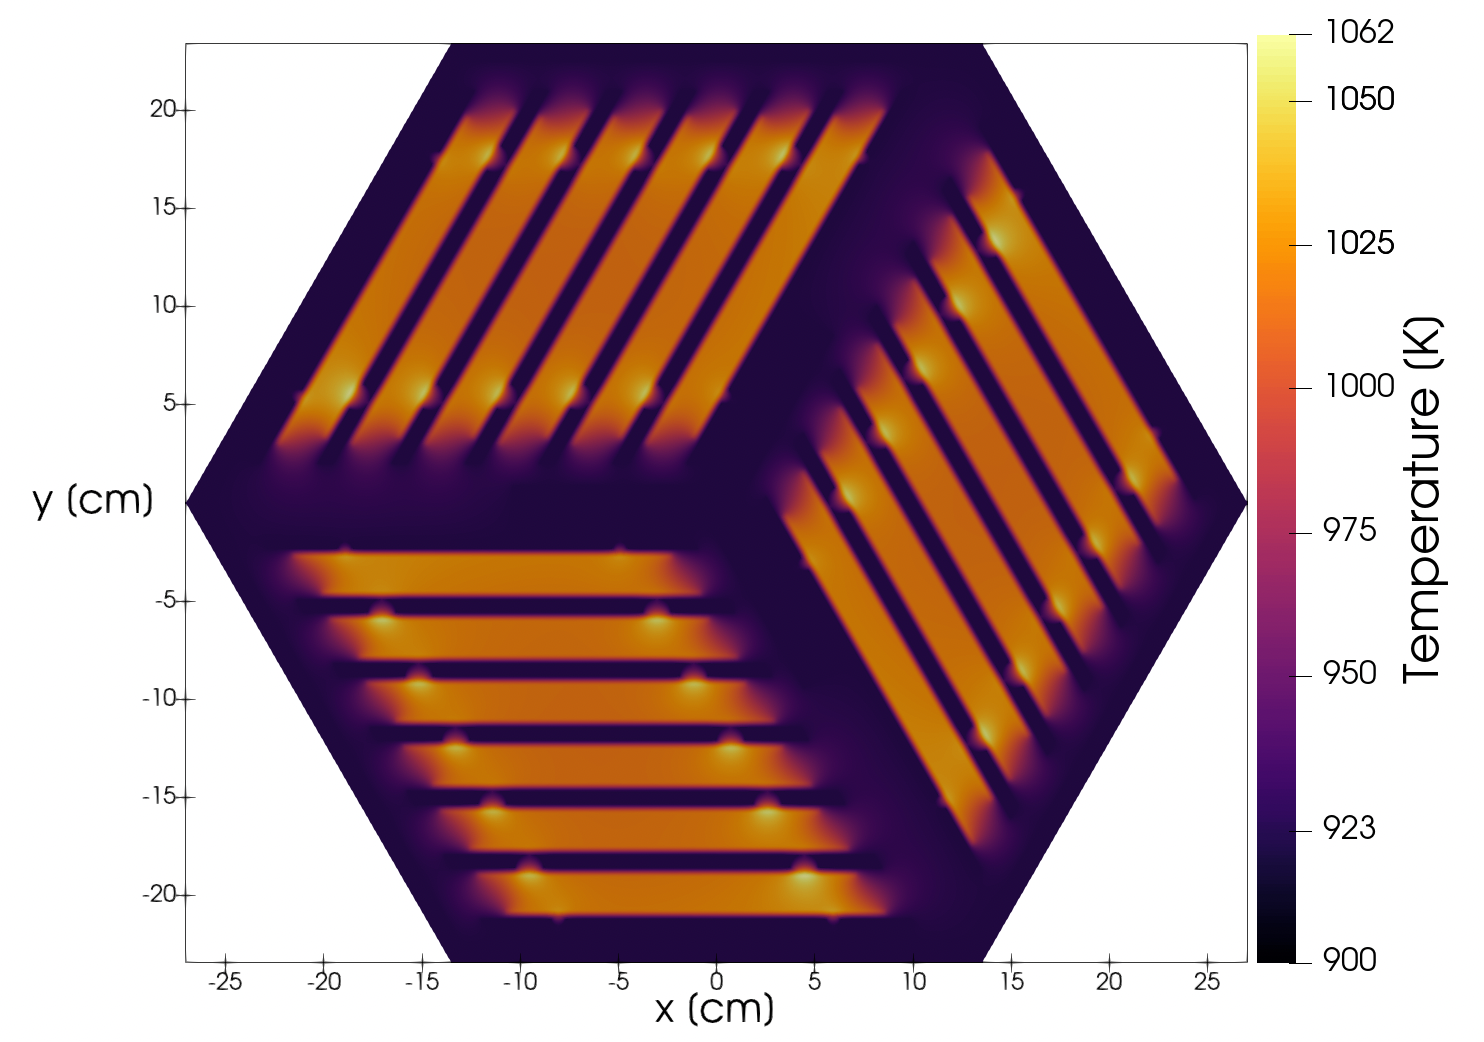
\includegraphics[width=\linewidth]{../docs/figures/benchmark-temperature-model.png} 
                \caption{2D temperature distribution in the \acrfull{AHTR}
                full assembly generated by Moltres.}
            \end{figure}
        \end{column}
        \begin{column}{0.4\textwidth} 
            \begin{block}{Results}
                \begin{itemize}
                    \item Average temperature distribution across the fuel planks are 
                    $\sim 1025K$
                    \item Average temperature of graphite structure is $\sim 935K$
                    \item Temperature peaks at 1062K in the fuel stripes near the spacers
                    \item This is due to the spacers displacing coolant and providing extra 
                    moderation 
                \end{itemize}
            \end{block}
        \end{column}
        \end{columns}
\end{frame}

\subsection{FHR Benchmark + AHTR Moltres Temperature Model: Summary}
\begin{frame}
    \frametitle{FHR Benchmark + AHTR Model Development: Summary}
    \begin{block}{Major Takeaways}
        \begin{itemize}
            \item AHTR has passive safety behavior with negative temperature coeffcients
            \item Increased fuel packing does not always correspond with increased 
            $k_{eff}$ due to self-shielding effects 
            \item These results hint at the possibility of minimizing fuel required by 
            optimizing for heterogenous fuel distributions within the core
            \item AHTR temperature peaks in the fuel stripes near the spacers 
        \end{itemize}
    \end{block}
    \begin{block}{I Successfully Completed AHTR Model Development Research Objectives}
        \begin{itemize}
            \item I participated in the OECD-NEA's FHR Benchmark Phases I-A and I-B
            \item I modeled the \gls{AHTR}'s temperature distribution 
        \end{itemize}
    \end{block}
\end{frame}
